\chapter{Результаты тестирования и оценка эффективности разработанного алгоритма} \label{chapt4}

Практическая реализация алгоритма была испытана на суперкомпьютере Ломоносов.
На рисунке \ref{img:a1} представлена зависимость времени от количества
используемых процессов на входной последовательности из 10 миллионов нуклеотидных
пар.


\begin{figure}[h]
\center{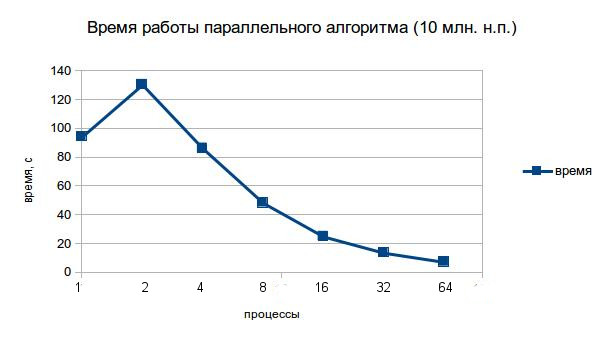
\includegraphics[width=0.5\linewidth]{image/1.jpg}}
\caption{Время работы параллельного алгоритма}
\label{img:a1}  
\end{figure}

\begin{figure}[h]
\center{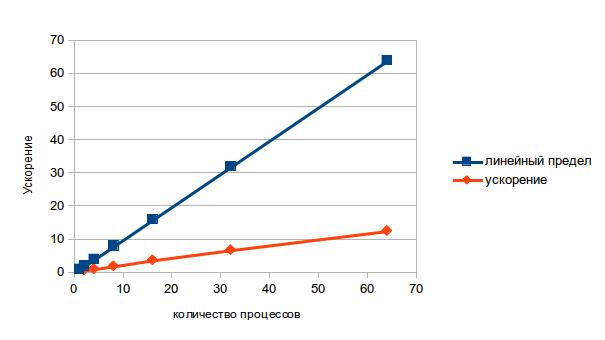
\includegraphics[width=0.5\linewidth]{image/2.jpg}}
\caption{Отклонение от максимального линейного ускорения}
\label{img:a2}  
\end{figure}

\clearpage


На рисунке \ref{img:a4} показано изменение в работе программы по сравнению
с первой версией. Вторая версия работает немного быстрее (в среднем на 10-20\%).
\begin{figure}[h]
\center{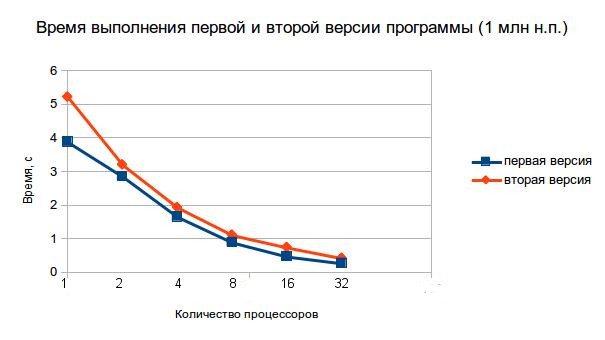
\includegraphics[width=0.5\linewidth]{image/4.jpg}}
\caption{Пример гомологической матрицы}
\label{img:a4}  
\end{figure}

Однако, как мы можем наблюдать на рисунке \ref{img:a5} вторая версия программы
при слишком большом количестве процессов начинает расти во времени. Связано это прежде всего с тем, что вторая программа
использует больше пересылок сообщений.
\begin{figure}[h]
\center{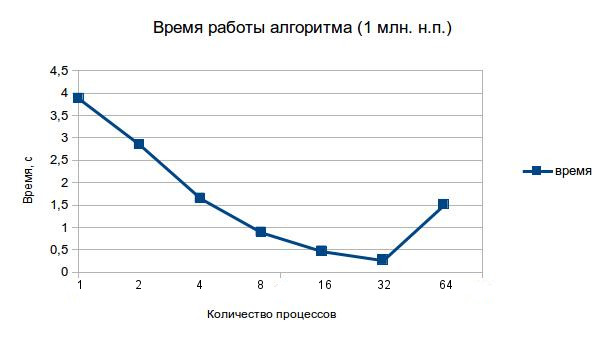
\includegraphics[width=0.5\linewidth]{image/5.jpg}}
\caption{Пример гомологической матрицы}
\label{img:a5}  
\end{figure}

На рисунке \ref{img:a6} представлена гемологическая матрица, полученная в ходе
работы программы на последовательности из 1 миллиона нуклеотидных пар.
\begin{figure}[h]
\center{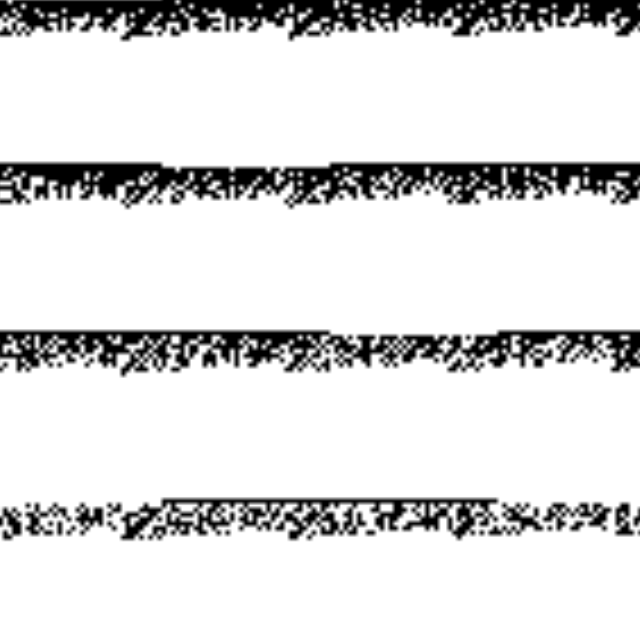
\includegraphics[width=0.5\linewidth]{image/6.png}}
\caption{Пример гомологической матрицы}
\label{img:a6}  
\end{figure}


\clearpage
